
\serie{Equations}

\begin{exercice}
\begin{enumerate}
\item Le nombre 2 est-il solution de l'équation\\
 $5x+1=2x+7$?
\item Le nombre $\dfrac{1}{2}$ est-il solution de l'équation\\ $3x-8=5x-11$?
\end{enumerate}
\end{exercice}


\begin{exercice}
Résoudre les équations suivantes:

\renewcommand{\arraystretch}{0.8}
\begin{tabular}{p{4cm}p{4cm}}
(a) $5x=3x+3$ & (b) $8x=12x+4$\\
&\\
(c) $4-7y=10y$ & (d) $7x+1=4-x$\\
&\\
(e) $2+3x=7+3x$ & (f) $-x=-8x-3,4$\\
&\\
(g) $5x+1=5x-1$ & (h) $5x=0$\\
\end{tabular}
\end{exercice}

\begin{exercice}
Résoudre les équations suivantes:

\renewcommand{\arraystretch}{0.8}
\begin{tabular}{p{6cm}p{1cm}}
(a) $7x-(5x+3)=5(x-3)+2$\\
&\\
(b) $4y+3(4y-2)=3(y+1)$\\
&\\
(c) $\dfrac{x}{5}-\dfrac{3x-2}{15}=\dfrac{1-x}{3}$\\
&\\
(d) $-4=\dfrac{-4x+30}{5}$\\
&\\
(e) $\dfrac{2x}{7}+\dfrac{3}{14}=\dfrac{x}{7}-\dfrac{1}{14}$\\
&\\
(f) $\dfrac{2}{5}x-\dfrac{1}{9}=\dfrac{3}{9}x+\dfrac{4}{5}$\\
\end{tabular}
\end{exercice}

\serie{Equations et problèmes}

\begin{exercice}
En multipliant un nombre par 12, on l’augmente de 253.\\
Quel est ce nombre?
\end{exercice}

\begin{exercice}
Le quadruple d’un nombre, diminué de 7, est égal au double de ce nombre, augmenté de 19.\\
Quel est ce nombre?
\end{exercice}


\begin{exercice}
Une personne a dépensé le tiers de son argent, puis le cinquième de l’argent restant et il lui reste encore 14 CHF.\\
Combien d’argent avait-elle initialement ?
\end{exercice}

\begin{exercice}
Combien y a-t-il d'élèves dans une classe sachant que le tiers travaille, deux cinquièmes bavardent et les huit qui restent somnolent?
\end{exercice}


\begin{exercice}
Le ciné-club d'une ville propose deux tarifs :
\begin{description}
\item Tarif A : une carte d'adhésion pour l'année coûtant 63 CHF, puis 4,5 CHF par séance;
\item Tarif B : 15 CHF par séance sans carte d'adhésion.
\end{description}

\begin{enumerate}
\item Calculer, pour chaque tarif, le prix payé pour 8 séances.
\item On appelle $x$ le nombre de séances. Exprimer en fonction de $x$ le prix payé avec le tarif A, puis avec le tarif B.
\item Quel est le nombre de séances pour lequel le tarif A est égal au tarif B ?
\end{enumerate}
\end{exercice}

\begin{exercice}
Quentin pense à un nombre, lui ajoute 11, multiplie le tout par 3 et au résultat obtenu il retranche 3. Joey obtient 51. Quel est le nombre de départ ?
\end{exercice}

\serie{Intervalles}

\begin{exercice}
Ecrire sous forme d’intervalle les inégalités ci-dessous et dessiner ces intervalles sur la droite réelle.\\

\renewcommand{\arraystretch}{0.8}
\begin{tabular}{p{4cm}p{4cm}}
(a) $-5\leq x \leq 2$ & (b) $-2 < x < 4$\\
&\\
(c) $0<x<7$ & (d) $-6 \leq x < 0$\\
&\\
(e) $x<-2$ & (f) $1<x$\\
&\\
(g) $x<0$ ou $4<x<10$ & (h) $x<3$ ou $x\geq 4$\\
&\\
(i) $x<5$ et $x\geq 4$ & (j) $x\geq -3$ et $x< 4$\\
\end{tabular}
\end{exercice}

\begin{exercice}
Ecrire sous forme d’inégalités et d’intervalles chacun des dessins ci-dessous.\\

\renewcommand{\arraystretch}{0.8}
\begin{tabular}{p{6cm}p{1cm}}
(a) 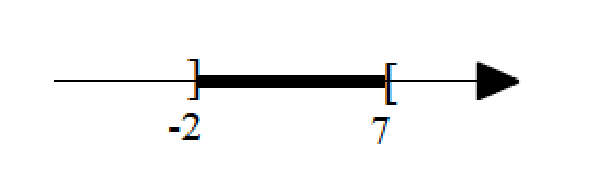
\includegraphics[scale=0.5]{I1}
 &\\
 (b) 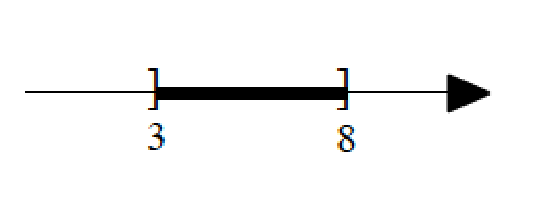
\includegraphics[scale=0.5]{I2}
&\\
(c) 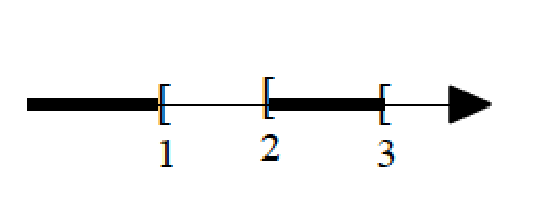
\includegraphics[scale=0.5]{I3}
\end{tabular}
\end{exercice}

\serie{Inéquations}

\begin{exercice}
Résoudre les inéquations suivantes:\\

\renewcommand{\arraystretch}{0.8}
\begin{tabular}{p{4cm}p{4cm}}
(a) $7x-8 > 6$ & (b) $4x+9>-21$\\
&\\
(c) $4-9x<7$ & (d) $2-6x\geq26$\\
&\\
(e) $2+7x>16$ & (f) $12>3-3x$\\
\end{tabular}
\end{exercice}

\begin{exercice}
Résoudre les inéquations suivantes:\\

\renewcommand{\arraystretch}{0.8}
\begin{tabular}{p{4cm}p{4cm}}
(a) $5x-7 > 11x+9$ & (b) $5x+5<5x$\\
&\\
(c) $2(4x-1)\leq 3x-6$ & (d) $2x-4 \geq 7-8x$\\
&\\
(e) $2-5x\geq 3(x-9)$ & (f) $\dfrac{1}{2}x-5>\dfrac{1}{4}x+3$\\
\end{tabular}
\end{exercice}

\begin{exercice}
Résoudre les inéquations suivantes:\\

\renewcommand{\arraystretch}{0.8}
\begin{tabular}{p{6cm}p{1cm}}
(a) $3(x+1)-x\leq1+2(1+x)$\\
&\\
(b) $-\dfrac{3}{5}x-6 < - \dfrac{2}{5}x+7$\\
&\\
(c) $-3(2-7x)+8-(3-3x)\geq 7-(3+5x)$\\
&\\
(d) $\dfrac{1}{5}-\dfrac{4}{3}\geq2\left( 1-\dfrac{5}{6}x\right) $\\

\end{tabular}
\end{exercice}

\begin{exercice}
Résoudre les inéquations suivantes:\\

\renewcommand{\arraystretch}{0.8}
\begin{tabular}{p{6cm}p{1cm}}
(a) $2x-(3x+4)\geq8x-7$\\
&\\
(b) $4+3(4x-5)\leq5-(7-2x)$\\
&\\
(c) $9-(3+7x)<2x+3(x-4)$\\
&\\
(d) $2x-\dfrac{2}{3}<2-\dfrac{x+1}{3}$\\

\end{tabular}
\end{exercice}

\begin{exercice}
\begin{enumerate}
\item Résoudre l'inéquation: $2x-7(3x-2)\leq 34 - 9 x$ et représenter graphiquement les solutions.
\item Résoudre l'inéquation: $6(3x-5) < 9-3(1-2x)$ et représenter graphiquement les solutions.
\item En utilisant les résultats précédents, représenter graphiquement les valeurs de $x$ qui vérifient: $2x-7(3x-2)\leq 34 - 9 x$ et $6(3x-5) < 9-3(1-2x)$.
\end{enumerate}
\end{exercice}

\serie{Inéquations et problèmes}

\begin{exercice}
La société Allo propose un abonnement téléphonique de 98 CHF par mois et1,30 CHF par minute de communication. 

La société Lalo propose un abonnement téléphonique de 95 CHF par mois et 1,45 CHF  par minute de communication.

On désigne par $x$  le nombre de minutes de communication par mois.

\begin{enumerate}
\item Exprimer en fonction de x  le montant d’une facture de Allo, puis le montant d’une facture de Lalo.
\item Pour quelles durées de communications mensuelles a-t-on intérêt à choisir Allo ?
\end{enumerate}
\end{exercice}

\begin{exercice}
Une entreprise de recherche emploie 27 informaticiens et 15 mathématiciens. 

On envisage d’embaucher le même nombre $x$  d’informaticiens et de mathématiciens.

Combien faut-il embaucher de spécialistes de chaque sorte pour que le nombre de mathématiciens soit au moins égal aux deux tiers du nombre d’informaticiens ?
\end{exercice}

\begin{exercice}
La longueur d’un rectangle dépasse de 7 dm sa largeur. 

On sait que son périmètre est compris entre 20 dm et 26 dm. 

Que peut-on dire au sujet de sa largeur ? 
\end{exercice}

\begin{exercice}
Paul a 32 ans et Mafalda a 5 ans. 

Pendant combien d’années l’âge de Paul restera-t-il plus grand que quatre fois celui de Mafalda ?  
\end{exercice}